\documentclass[12pt,a4paper]{article}
\usepackage[utf8]{inputenc}
\usepackage[english]{babel}
\usepackage{geometry}
\usepackage{fancyhdr}
\usepackage{graphicx}
\usepackage{longtable}
\usepackage{array}
\usepackage{booktabs}
\usepackage{xcolor}
\usepackage{hyperref}
\usepackage{listings}
\usepackage{enumitem}

\geometry{margin=1in}
\pagestyle{fancy}
\fancyhf{}
\rhead{\thepage}
\lhead{HIV Clinic RDS}

\title{\textbf{Requirement \& Design Specification\\HIV Clinic Appointment Booking System}}
\author{Version: 1.0}
\date{January 2025}

\begin{document}

\maketitle
\thispagestyle{empty}

\newpage

\section*{Record of Changes}

\begin{longtable}{|p{2cm}|p{2cm}|p{1cm}|p{3cm}|p{6cm}|}
\hline
\textbf{Version} & \textbf{Date} & \textbf{A*M, D} & \textbf{In charge} & \textbf{Change Description} \\
\hline
V1.0 & 07/01/2025 & A & Development Team & Initial HIV Clinic System RDS document based on implemented codebase \\
\hline
\end{longtable}

\textit{*A - Added M - Modified D - Deleted}

\newpage

\tableofcontents

\newpage

\section{Overview}

\subsection{User Requirements}

\subsubsection{Actors}

The HIV Clinic Appointment Booking System involves four main actors who interact with the system to perform various healthcare-related tasks:

\begin{longtable}{|p{1cm}|p{3cm}|p{10cm}|}
\hline
\textbf{\#} & \textbf{Actor} & \textbf{Description} \\
\hline
1 & Patient & Registered HIV patients who book appointments, manage their medical records, view treatment information, and receive medication reminders \\
\hline
2 & Doctor & HIV/AIDS specialists and healthcare providers who manage patient appointments, update medical records, prescribe ARV treatments, and access patient information during consultations \\
\hline
3 & Admin & System administrators who manage user accounts, system settings, and have full access to all system functionalities for maintenance and oversight \\
\hline
4 & Manager & Healthcare facility managers who oversee operations, generate reports, and manage clinic resources and staff schedules \\
\hline
\end{longtable}

\subsubsection{Use Cases}

\paragraph{a. Diagram(s)}

\begin{figure}[H]
\centering
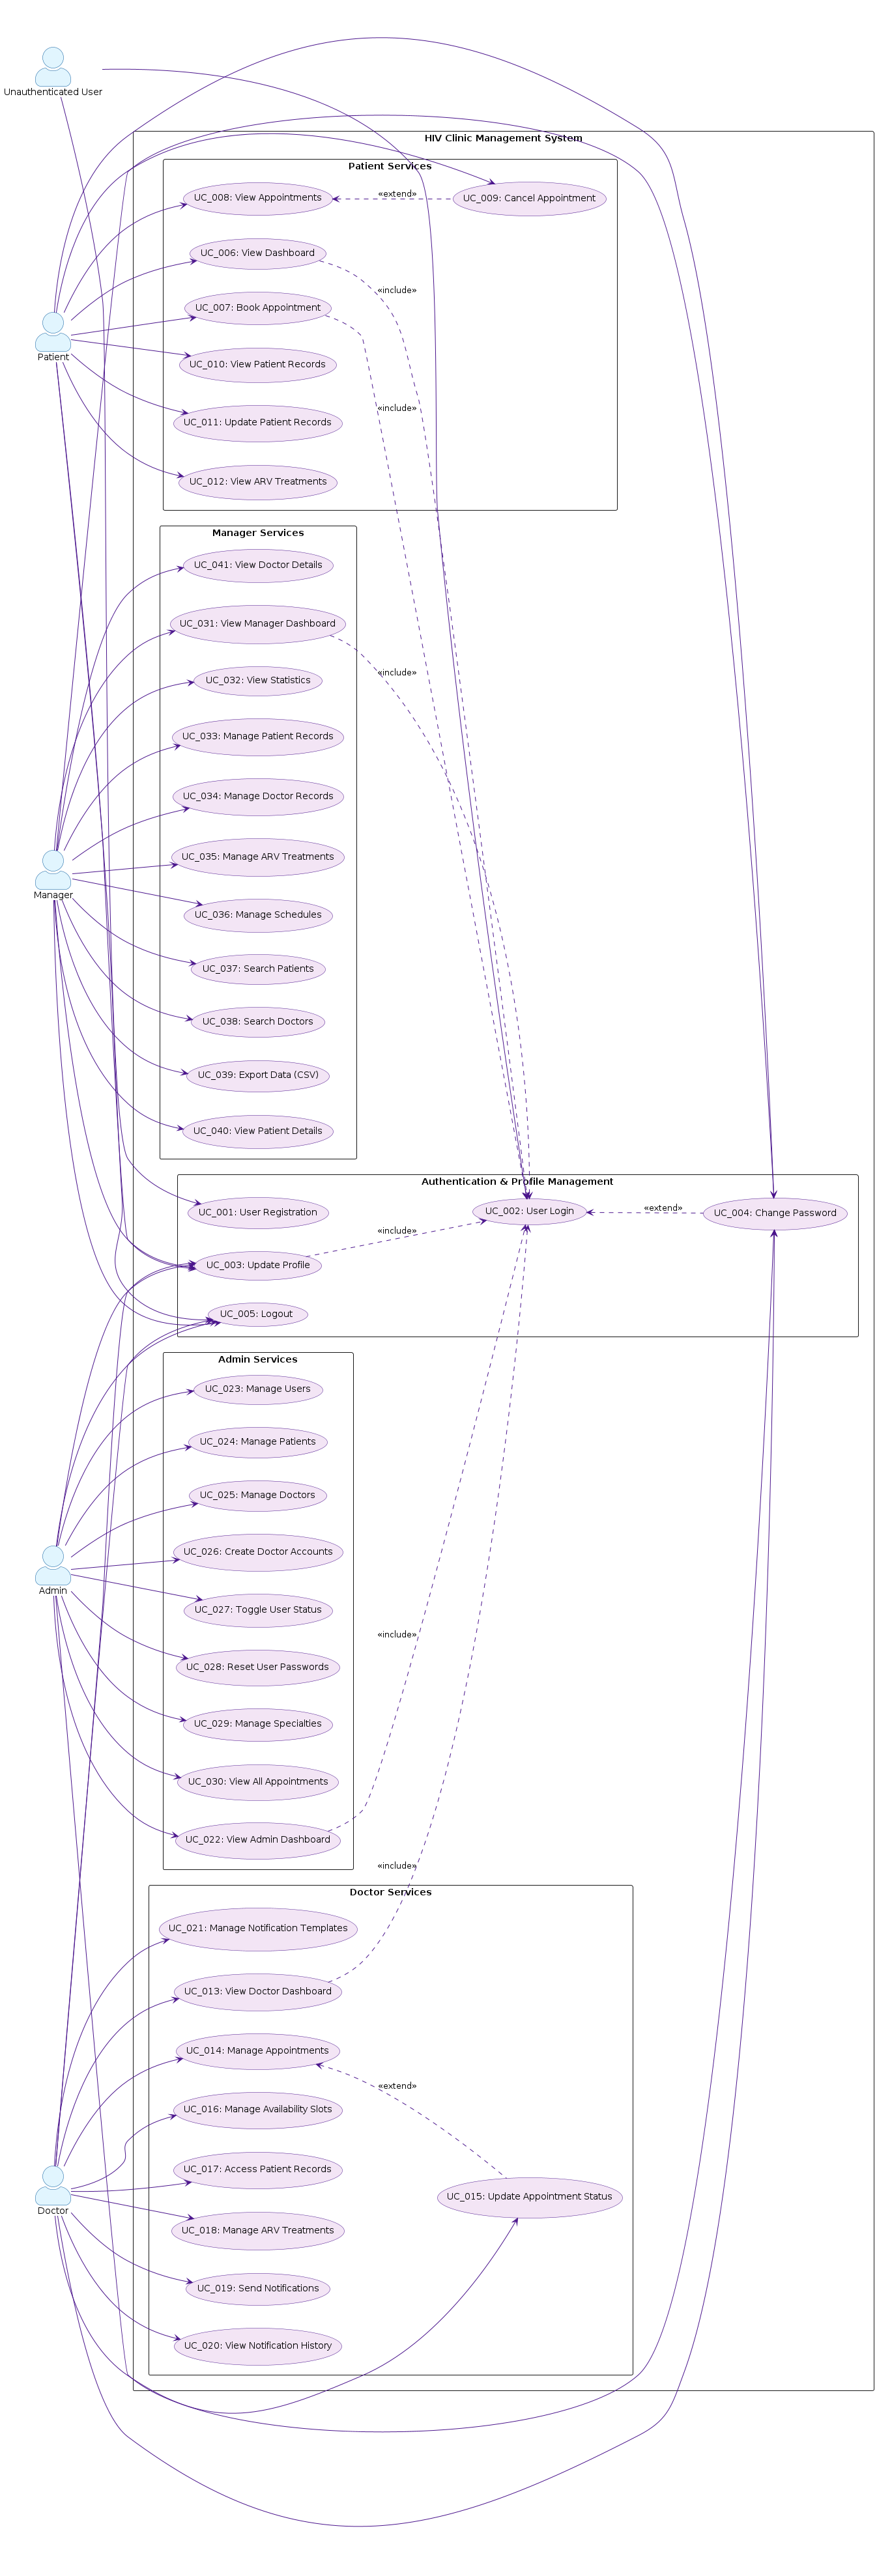
\includegraphics[width=0.9\textwidth]{diagrams/use_case_diagram.png}
\caption{HIV Clinic Management System Use Case Diagram}
\label{fig:use-case-diagram}
\end{figure}

The system provides comprehensive use cases covering patient care, appointment management, and administrative functions for an HIV clinic environment.

\paragraph{b. Descriptions}

\begin{longtable}{|p{1cm}|p{3cm}|p{3cm}|p{7cm}|}
\hline
\textbf{ID} & \textbf{Feature} & \textbf{Use Case} & \textbf{Use Case Description} \\
\hline
UC-001 & User Management & User Registration & New users (patients/doctors) create accounts with role-based access to the HIV clinic system \\
\hline
UC-002 & Authentication & User Login & Existing users authenticate using username/password with JWT token-based security \\
\hline
UC-003 & Profile Management & Update Profile & Users update personal information, contact details, and profile images \\
\hline
UC-004 & Appointment Management & Book Appointment & Patients schedule appointments with available doctors based on doctor availability slots \\
\hline
UC-005 & Doctor Operations & Manage Availability & Doctors create, update, and manage their availability time slots for patient appointments \\
\hline
UC-006 & Appointment Management & Cancel Appointment & Patients or doctors cancel scheduled appointments with cancellation reasons \\
\hline
UC-007 & Patient Care & Manage Patient Records & Doctors access and update patient medical records including history, allergies, and current medications \\
\hline
UC-008 & HIV Treatment & ARV Treatment Management & Doctors manage HIV antiretroviral treatment regimens, monitor adherence, and track side effects \\
\hline
UC-009 & Medication Management & Medication Routine Management & Doctors create medication schedules and patients receive automated reminders for ARV adherence \\
\hline
UC-010 & Notification System & Appointment Reminders & System sends automated reminders to patients for upcoming appointments (24-hour, 1-hour, 30-minute) \\
\hline
UC-011 & Notification System & Medication Reminders & System sends daily medication reminders to patients based on their prescribed ARV routine \\
\hline
UC-012 & Patient Privacy & Privacy Settings & Patients control the visibility of their medical information and set privacy preferences \\
\hline
\end{longtable}

\subsection{Overall Functionalities}

\subsubsection{Screens Flow}

The HIV Clinic system provides role-based screen flows ensuring appropriate access to sensitive medical information:

\begin{itemize}
    \item \textbf{Patient Flow}: Login → Patient Dashboard → Book Appointment → View Medical Records → Medication Reminders
    \item \textbf{Doctor Flow}: Login → Doctor Dashboard → Manage Availability → View Patient Records → Update Treatment Plans
    \item \textbf{Admin Flow}: Login → Admin Dashboard → User Management → System Settings → Reports
    \item \textbf{Manager Flow}: Login → Manager Dashboard → Clinic Operations → Staff Management → Analytics
\end{itemize}

\begin{figure}[H]
\centering
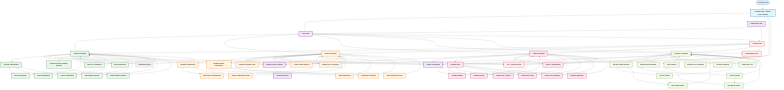
\includegraphics[width=0.9\textwidth]{diagrams/user_interface_flow.png}
\caption{User Interface Flow Diagram}
\label{fig:ui-flow-diagram}
\end{figure}

\subsubsection{Screen Descriptions}

\begin{longtable}{|p{1cm}|p{3cm}|p{3cm}|p{7cm}|}
\hline
\textbf{\#} & \textbf{Feature} & \textbf{Screen} & \textbf{Description} \\
\hline
1 & Authentication & Login Screen & Secure login with username/password authentication and JWT token generation \\
\hline
2 & Authentication & Registration Screen & User registration with role selection, profile information, and email verification \\
\hline
3 & Patient Dashboard & Patient Home & Overview of upcoming appointments, medication reminders, and treatment status \\
\hline
4 & Appointment Management & Book Appointment & Search available doctors, view time slots, and schedule appointments \\
\hline
5 & Appointment Management & My Appointments & View scheduled, completed, and cancelled appointments with details \\
\hline
6 & Doctor Dashboard & Doctor Home & Overview of daily appointments, patient notifications, and availability management \\
\hline
7 & Doctor Operations & Availability Management & Create, update, and manage doctor availability time slots \\
\hline
8 & Patient Records & Medical Records & Comprehensive patient medical history, allergies, current medications, and emergency contacts \\
\hline
9 & ARV Treatment & Treatment Management & HIV treatment regimens, adherence tracking, and side effect monitoring \\
\hline
10 & Medication Management & Medication Routine & Daily medication schedules, dosage information, and reminder settings \\
\hline
11 & Notification System & Notification Center & View and manage appointment reminders and medication alerts \\
\hline
12 & Admin Panel & User Management & Manage user accounts, roles, and system permissions \\
\hline
\end{longtable}

\subsubsection{Screen Authorization}

\begin{longtable}{|p{4cm}|p{2cm}|p{2cm}|p{2cm}|p{2cm}|}
\hline
\textbf{Screen} & \textbf{Patient} & \textbf{Doctor} & \textbf{Admin} & \textbf{Manager} \\
\hline
Login Screen & X & X & X & X \\
\hline
Registration Screen & X & X & X & X \\
\hline
Patient Dashboard & X & & & \\
\hline
\quad View Own Records & X & & & \\
\hline
\quad Update Own Profile & X & & & \\
\hline
\quad Book Appointments & X & & & \\
\hline
Doctor Dashboard & & X & & \\
\hline
\quad Manage Availability & & X & & \\
\hline
\quad View Patient Records & & X & X & \\
\hline
\quad Update Treatment Plans & & X & & \\
\hline
Admin Dashboard & & & X & \\
\hline
\quad User Management & & & X & \\
\hline
\quad System Settings & & & X & \\
\hline
Manager Dashboard & & & & X \\
\hline
\quad Generate Reports & & & X & X \\
\hline
\quad View Analytics & & & X & X \\
\hline
Appointment Management & X & X & X & X \\
\hline
\quad Cancel Appointments & X & X & X & \\
\hline
Notification System & X & X & X & X \\
\hline
\end{longtable}

\subsubsection{Non-UI Functions}

\begin{longtable}{|p{1cm}|p{4cm}|p{4cm}|p{5cm}|}
\hline
\textbf{\#} & \textbf{Feature} & \textbf{System Function} & \textbf{Description} \\
\hline
1 & Notification Scheduling & Automated Reminder Service & Background service that schedules and sends appointment and medication reminders based on configured templates \\
\hline
2 & Security & JWT Token Management & Automatic token generation, validation, and refresh for secure API access \\
\hline
3 & Data Validation & Input Sanitization & Server-side validation and sanitization of all user inputs to prevent SQL injection and XSS attacks \\
\hline
4 & Audit Logging & Activity Tracking & Automatic logging of user actions, login attempts, and data modifications for security and compliance \\
\hline
5 & Database Management & Automated Backups & Scheduled database backups and maintenance operations \\
\hline
6 & Email Service & SMTP Integration & Email delivery service for notifications and system communications \\
\hline
\end{longtable}

\subsection{System High Level Design}

\subsubsection{Database Design}

\paragraph{a. Database Schema}

The HIV Clinic system uses Microsoft SQL Server with the following core tables:

\begin{itemize}
    \item \textbf{Users}: Central user management with role-based access
    \item \textbf{Roles}: System roles (Patient, Doctor, Admin, Manager)
    \item \textbf{PatientProfiles}: Extended patient information
    \item \textbf{DoctorProfiles}: Extended doctor information with specialties
    \item \textbf{Appointments}: Appointment scheduling and management
    \item \textbf{DoctorAvailabilitySlots}: Doctor availability management
    \item \textbf{PatientRecords}: Medical records and patient history
    \item \textbf{ARVTreatments}: HIV antiretroviral treatment tracking
    \item \textbf{MedicationRoutines}: Daily medication schedules
    \item \textbf{Notifications}: System notification management
    \item \textbf{NotificationTemplates}: Reusable notification templates
\end{itemize}

\paragraph{b. Table Descriptions}

\begin{longtable}{|p{1cm}|p{3cm}|p{10cm}|}
\hline
\textbf{No} & \textbf{Table} & \textbf{Description} \\
\hline
01 & Users & Central user authentication and profile management table storing username, password hash, email, and role associations \\
& & - Primary keys: UserID \\
& & - Foreign keys: RoleID (references Roles) \\
\hline
02 & Roles & System role definitions for access control \\
& & - Primary keys: RoleID \\
& & - Contains: Patient, Doctor, Admin, Manager roles \\
\hline
03 & PatientProfiles & Extended patient information including demographics and privacy settings \\
& & - Primary keys: PatientProfileID \\
& & - Foreign keys: UserID (references Users) \\
\hline
04 & DoctorProfiles & Doctor professional information including specialties and qualifications \\
& & - Primary keys: DoctorProfileID \\
& & - Foreign keys: UserID (references Users), SpecialtyID (references Specialties) \\
\hline
05 & Appointments & Appointment scheduling between patients and doctors \\
& & - Primary keys: AppointmentID \\
& & - Foreign keys: PatientUserID, DoctorUserID (references Users), AvailabilitySlotID \\
\hline
06 & DoctorAvailabilitySlots & Doctor availability time slot management \\
& & - Primary keys: AvailabilitySlotID \\
& & - Foreign keys: DoctorUserID (references Users) \\
\hline
07 & PatientRecords & Comprehensive medical records including history, allergies, medications \\
& & - Primary keys: RecordID \\
& & - Foreign keys: PatientUserID (references Users) \\
\hline
08 & ARVTreatments & HIV antiretroviral treatment regimens and monitoring \\
& & - Primary keys: ARVTreatmentID \\
& & - Foreign keys: PatientUserID, DoctorUserID (references Users), AppointmentID \\
\hline
09 & MedicationRoutines & Daily medication schedules and reminder configurations \\
& & - Primary keys: RoutineID \\
& & - Foreign keys: PatientUserID, DoctorUserID (references Users), ARVTreatmentID \\
\hline
10 & Notifications & System notifications for appointments and medication reminders \\
& & - Primary keys: NotificationID \\
& & - Foreign keys: UserID (references Users), templateId (references NotificationTemplates) \\
\hline
11 & NotificationTemplates & Reusable notification message templates \\
& & - Primary keys: templateId \\
& & - Contains: appointment reminder, medication reminder, and system notification templates \\
\hline
\end{longtable}

\subsubsection{Code Packages}

The HIV Clinic system follows a layered Spring Boot architecture:

\begin{longtable}{|p{1cm}|p{4cm}|p{9cm}|}
\hline
\textbf{No} & \textbf{Package} & \textbf{Description} \\
\hline
01 & com.hivclinic.controller & REST API controllers handling HTTP requests for appointments, authentication, patient records, doctor operations, and notifications \\
\hline
02 & com.hivclinic.service & Business logic layer containing services for appointment management, user authentication, patient care, ARV treatment, and notification scheduling \\
\hline
03 & com.hivclinic.repository & Data access layer with JPA repositories for database operations \\
\hline
04 & com.hivclinic.model & Entity classes representing database tables including User, Appointment, PatientRecord, ARVTreatment, and Notification models \\
\hline
05 & com.hivclinic.dto & Data Transfer Objects for request/response handling and API communication \\
\hline
06 & com.hivclinic.config & Configuration classes for security (JWT), database, and application settings \\
\hline
07 & com.hivclinic.exception & Custom exception handling for application-specific errors \\
\hline
08 & com.hivclinic.validation & Input validation and sanitization utilities \\
\hline
\end{longtable}

\subsubsection{Data Flow Architecture}

\begin{figure}[H]
\centering
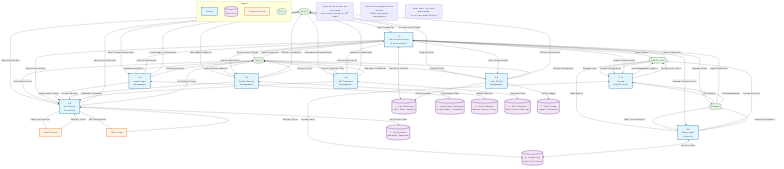
\includegraphics[width=0.9\textwidth]{diagrams/data_flow_diagram.png}
\caption{System Data Flow Diagram}
\label{fig:data-flow-diagram}
\end{figure}

\section{Requirement Specifications}

\subsection{Authentication \& User Management}

\subsubsection{UC-001\_User Registration}

\paragraph{a. Functionalities}

\textbf{UC ID and Name:} UC-001 User Registration

\textbf{Created By:} Development Team

\textbf{Date Created:} January 2025

\textbf{Primary Actor:} Guest User (future Patient/Doctor)

\textbf{Secondary Actors:} System Administrator

\textbf{Trigger:} New user accesses registration page and submits registration form

\textbf{Description:} New users register for accounts in the HIV clinic system with role-based access. The system validates user information, creates secure accounts, and establishes appropriate permissions.

\textbf{Preconditions:}
\begin{itemize}
    \item User has valid email address
    \item Username is unique in the system
    \item Password meets security requirements
\end{itemize}

\textbf{Postconditions:}
\begin{itemize}
    \item User account created with encrypted password
    \item Role assigned based on registration type
    \item User profile initialized
    \item Account activation email sent
\end{itemize}

\textbf{Normal Flow:}
\begin{enumerate}
    \item User accesses registration screen
    \item User enters username, email, password, and confirms password
    \item User selects role (Patient/Doctor)
    \item User provides additional profile information
    \item System validates input data
    \item System checks username and email uniqueness
    \item System creates user account with encrypted password
    \item System assigns appropriate role
    \item System creates corresponding profile record
    \item System sends confirmation response
\end{enumerate}

\textbf{Alternative Flows:}
\begin{itemize}
    \item \textbf{1.1 Doctor Registration:} Additional validation for medical credentials and specialty selection
\end{itemize}

\textbf{Exceptions:}
\begin{itemize}
    \item \textbf{1.0.E1:} Username already exists - System displays error message
    \item \textbf{1.0.E2:} Email already registered - System displays error message
    \item \textbf{1.0.E3:} Password confirmation mismatch - System requests password re-entry
    \item \textbf{1.0.E4:} Invalid email format - System displays validation error
\end{itemize}

\textbf{Priority:} Must Have

\textbf{Frequency of Use:} Low frequency, primarily during initial system rollout

\textbf{Business Rules:} BR-001, BR-002, BR-003

\paragraph{b. Business Rules}

\begin{longtable}{|p{2cm}|p{4cm}|p{8cm}|}
\hline
\textbf{ID} & \textbf{Business Rule} & \textbf{Business Rule Description} \\
\hline
BR-001 & Password Security & User passwords must be hashed using BCrypt with minimum 8 characters, including uppercase, lowercase, and numbers \\
\hline
BR-002 & Unique Credentials & Username and email must be unique across the entire system \\
\hline
BR-003 & Role Validation & Doctor registrations require additional verification of medical credentials \\
\hline
\end{longtable}

\subsubsection{UC-002\_User Login}

\paragraph{a. Functional Description}

\textbf{UC ID and Name:} UC-002 User Login

\textbf{Created By:} Development Team

\textbf{Date Created:} January 2025

\textbf{Primary Actor:} Registered User (Patient/Doctor/Admin/Manager)

\textbf{Secondary Actors:} Authentication Service

\textbf{Trigger:} User attempts to access the system or protected resources

\textbf{Description:} Registered users authenticate using username/password credentials to access role-appropriate system features. The system validates credentials and provides JWT tokens for secure session management.

\textbf{Preconditions:}
\begin{itemize}
    \item User account exists and is active
    \item User has valid credentials
\end{itemize}

\textbf{Postconditions:}
\begin{itemize}
    \item User session established with JWT token
    \item User redirected to role-appropriate dashboard
    \item Login activity logged for security audit
\end{itemize}

\textbf{Normal Flow:}
\begin{enumerate}
    \item User accesses login screen
    \item User enters username and password
    \item System validates credentials against database
    \item System generates JWT token with role information
    \item System returns authentication response with token
    \item User redirected to appropriate dashboard
    \item System logs successful login activity
\end{enumerate}

\textbf{Alternative Flows:} None

\textbf{Exceptions:}
\begin{itemize}
    \item \textbf{2.0.E1:} Invalid credentials - System displays error message and logs failed attempt
    \item \textbf{2.0.E2:} Account inactive - System displays account status message
    \item \textbf{2.0.E3:} Multiple failed attempts - System temporarily locks account
\end{itemize}

\textbf{Priority:} Must Have

\textbf{Frequency of Use:} High - Daily usage by all system users

\textbf{Business Rules:} BR-004, BR-005, BR-006

\paragraph{b. Business Rules}

\begin{longtable}{|p{2cm}|p{4cm}|p{8cm}|}
\hline
\textbf{ID} & \textbf{Business Rule} & \textbf{Business Rule Description} \\
\hline
BR-004 & Session Management & JWT tokens expire after 24 hours and must be refreshed for continued access \\
\hline
BR-005 & Account Lockout & Account locked for 30 minutes after 5 consecutive failed login attempts \\
\hline
BR-006 & Audit Logging & All login attempts (successful and failed) are logged with timestamp, IP address, and user agent \\
\hline
\end{longtable}

\subsection{Appointment Management}

\subsubsection{UC-004\_Book Appointment}

\paragraph{a. Functional Description}

\textbf{UC ID and Name:} UC-004 Book Appointment

\textbf{Created By:} Development Team

\textbf{Date Created:} January 2025

\textbf{Primary Actor:} Patient

\textbf{Secondary Actors:} Doctor (availability provider)

\textbf{Trigger:} Patient initiates appointment booking process

\textbf{Description:} Patients book appointments with available doctors by selecting from available time slots. The system ensures no double-booking and automatically updates doctor availability.

\textbf{Preconditions:}
\begin{itemize}
    \item Patient is logged into the system
    \item Doctor has available time slots
    \item Patient has no conflicting appointments
\end{itemize}

\textbf{Postconditions:}
\begin{itemize}
    \item Appointment created with "Scheduled" status
    \item Doctor availability slot marked as booked
    \item Appointment confirmation sent to patient
    \item Automatic reminders scheduled
\end{itemize}

\textbf{Normal Flow:}
\begin{enumerate}
    \item Patient accesses appointment booking screen
    \item System displays list of available doctors
    \item Patient selects preferred doctor
    \item System displays available time slots for selected doctor
    \item Patient selects desired appointment time
    \item Patient provides appointment notes (optional)
    \item System validates appointment availability
    \item System creates appointment record
    \item System updates doctor availability slot
    \item System schedules automatic reminders
    \item System sends confirmation to patient
\end{enumerate}

\textbf{Alternative Flows:}
\begin{itemize}
    \item \textbf{4.1 Emergency Appointment:} Priority booking for urgent medical needs
\end{itemize}

\textbf{Exceptions:}
\begin{itemize}
    \item \textbf{4.0.E1:} Time slot no longer available - System refreshes available slots
    \item \textbf{4.0.E2:} Patient has conflicting appointment - System displays conflict warning
    \item \textbf{4.0.E3:} Maximum appointments per day exceeded - System enforces daily limit
\end{itemize}

\textbf{Priority:} Must Have

\textbf{Frequency of Use:} High - Multiple daily bookings expected

\textbf{Business Rules:} BR-007, BR-008, BR-009

\paragraph{b. Business Rules}

\begin{longtable}{|p{2cm}|p{4cm}|p{8cm}|}
\hline
\textbf{ID} & \textbf{Business Rule} & \textbf{Business Rule Description} \\
\hline
BR-007 & Appointment Limits & Patients limited to 3 active appointments at any time \\
\hline
BR-008 & Advance Booking & Appointments can be booked up to 30 days in advance \\
\hline
BR-009 & Default Duration & All appointments default to 30 minutes unless specified otherwise \\
\hline
\end{longtable}

\subsection{Patient Care Management}

\subsubsection{UC-007\_Manage Patient Records}

\paragraph{a. Functional Description}

\textbf{UC ID and Name:} UC-007 Manage Patient Records

\textbf{Created By:} Development Team

\textbf{Date Created:} January 2025

\textbf{Primary Actor:} Doctor

\textbf{Secondary Actors:} Patient, Admin

\textbf{Trigger:} Doctor accesses patient record during appointment or review

\textbf{Description:} Doctors access and update comprehensive patient medical records including medical history, allergies, current medications, and treatment notes. The system maintains complete audit trails of all record modifications.

\textbf{Preconditions:}
\begin{itemize}
    \item Doctor is authenticated with appropriate permissions
    \item Patient record exists in the system
    \item Doctor has legitimate medical reason for access
\end{itemize}

\textbf{Postconditions:}
\begin{itemize}
    \item Patient record updated with new information
    \item Modification audit trail created
    \item Patient notified of record updates (if enabled)
\end{itemize}

\textbf{Normal Flow:}
\begin{enumerate}
    \item Doctor searches for patient record
    \item System displays patient medical information
    \item Doctor reviews current medical history
    \item Doctor updates relevant medical information
    \item Doctor adds appointment notes
    \item System validates input data
    \item System saves record updates
    \item System creates audit log entry
    \item System confirms successful update
\end{enumerate}

\textbf{Alternative Flows:}
\begin{itemize}
    \item \textbf{7.1 Emergency Access:} Override access for emergency medical situations
    \item \textbf{7.2 Patient Self-Update:} Patients update non-clinical information
\end{itemize}

\textbf{Exceptions:}
\begin{itemize}
    \item \textbf{7.0.E1:} Access denied - Patient privacy settings prevent access
    \item \textbf{7.0.E2:} Record locked - Another doctor currently editing
    \item \textbf{7.0.E3:} Invalid data - System validates medical information format
\end{itemize}

\textbf{Priority:} Must Have

\textbf{Frequency of Use:} High - Used during every patient consultation

\textbf{Business Rules:} BR-010, BR-011, BR-012

\paragraph{b. Business Rules}

\begin{longtable}{|p{2cm}|p{4cm}|p{8cm}|}
\hline
\textbf{ID} & \textbf{Business Rule} & \textbf{Business Rule Description} \\
\hline
BR-010 & Privacy Protection & Patient records can only be accessed by treating doctors or with explicit patient consent \\
\hline
BR-011 & Audit Requirements & All record access and modifications must be logged with doctor ID, timestamp, and reason \\
\hline
BR-012 & Data Retention & Patient records must be retained for minimum 7 years as per medical regulations \\
\hline
\end{longtable}

\subsection{Notification System}

\subsubsection{UC-010\_Appointment Reminders}

\paragraph{a. Functional Description}

\textbf{UC ID and Name:} UC-010 Appointment Reminders

\textbf{Created By:} Development Team

\textbf{Date Created:} January 2025

\textbf{Primary Actor:} System (Automated Service)

\textbf{Secondary Actors:} Patient, Notification Service

\textbf{Trigger:} Scheduled reminder time reached for upcoming appointment

\textbf{Description:} System automatically sends appointment reminders to patients at configured intervals (24 hours, 1 hour, 30 minutes) before scheduled appointments using notification templates.

\textbf{Preconditions:}
\begin{itemize}
    \item Appointment exists with scheduled date/time
    \item Patient has active notification preferences
    \item Notification templates configured
\end{itemize}

\textbf{Postconditions:}
\begin{itemize}
    \item Reminder notification sent to patient
    \item Notification status updated in database
    \item Delivery confirmation logged
\end{itemize}

\textbf{Normal Flow:}
\begin{enumerate}
    \item System scheduler identifies upcoming appointments
    \item System checks reminder intervals (24h, 1h, 30min)
    \item System selects appropriate notification template
    \item System personalizes message with patient/doctor details
    \item System sends notification via configured channels
    \item System logs notification delivery
    \item System updates reminder status
\end{enumerate}

\textbf{Alternative Flows:}
\begin{itemize}
    \item \textbf{10.1 SMS Reminder:} Send reminder via SMS for urgent notifications
    \item \textbf{10.2 Email Reminder:} Send detailed reminder via email
\end{itemize}

\textbf{Exceptions:}
\begin{itemize}
    \item \textbf{10.0.E1:} Delivery failure - System retries notification delivery
    \item \textbf{10.0.E2:} Patient opted out - System skips notification
    \item \textbf{10.0.E3:} Appointment cancelled - System cancels pending reminders
\end{itemize}

\textbf{Priority:} Should Have

\textbf{Frequency of Use:} High - Automated daily operations

\textbf{Business Rules:} BR-013, BR-014, BR-015

\paragraph{b. Business Rules}

\begin{longtable}{|p{2cm}|p{4cm}|p{8cm}|}
\hline
\textbf{ID} & \textbf{Business Rule} & \textbf{Business Rule Description} \\
\hline
BR-013 & Reminder Schedule & Appointment reminders sent at 24 hours, 1 hour, and 30 minutes before appointment \\
\hline
BR-014 & Template Usage & All notifications must use predefined templates for consistency \\
\hline
BR-015 & Opt-out Respect & System must respect patient notification preferences and opt-out requests \\
\hline
\end{longtable}

\section{Design Specifications}

\subsection{Authentication System}

\subsubsection{User Login}

This screen allows users to authenticate into the system with role-based access to appropriate functionalities.

\textbf{Related use cases:} UC-002 User Login

\paragraph{UI Design}

\begin{longtable}{|p{3cm}|p{3cm}|p{8cm}|}
\hline
\textbf{Field Name} & \textbf{Field Type} & \textbf{Description} \\
\hline
Username* & Text Box & User enters registered username or email address for authentication \\
\hline
Password* & Password Box & User enters password (masked input for security) \\
\hline
Login & Button & Submits authentication request to server \\
\hline
Register & Hyperlink & Redirects to user registration page for new users \\
\hline
Forgot Password? & Hyperlink & Initiates password reset process \\
\hline
\end{longtable}

\paragraph{Database Access}

\begin{longtable}{|p{3cm}|p{2cm}|p{9cm}|}
\hline
\textbf{Table} & \textbf{CRUD} & \textbf{Description} \\
\hline
Users & R & Verify username/email and password hash for authentication \\
\hline
Roles & R & Retrieve user role information for authorization \\
\hline
LoginActivity & C & Log login attempt for security audit \\
\hline
\end{longtable}

\paragraph{SQL Commands}

\begin{lstlisting}[language=SQL]
-- 1. Authenticate user credentials
SELECT u.UserID, u.Username, u.Email, u.IsActive, r.RoleName
FROM Users u 
INNER JOIN Roles r ON u.RoleID = r.RoleID
WHERE (u.Username = ? OR u.Email = ?) AND u.IsActive = 1

-- 2. Log login activity
INSERT INTO LoginActivity 
(UserID, UsernameAttempted, AttemptTime, IsSuccess, IPAddress, UserAgent)
VALUES (?, ?, GETDATE(), ?, ?, ?)
\end{lstlisting}

\subsection{Appointment Management}

\subsubsection{Appointment Booking}

This screen enables patients to book appointments with available doctors by selecting from available time slots.

\textbf{Related use cases:} UC-004 Book Appointment

\paragraph{UI Design}

\begin{longtable}{|p{3cm}|p{3cm}|p{8cm}|}
\hline
\textbf{Field Name} & \textbf{Field Type} & \textbf{Description} \\
\hline
Doctor Selection* & Dropdown & List of available doctors with specialties \\
\hline
Appointment Date* & Date Picker & Calendar widget for selecting appointment date \\
\hline
Available Time Slots* & Radio Buttons & Dynamic list of available time slots for selected doctor/date \\
\hline
Appointment Notes & Text Area & Optional notes about appointment purpose or concerns \\
\hline
Book Appointment & Button & Submit appointment booking request \\
\hline
Cancel & Button & Return to previous screen without booking \\
\hline
\end{longtable}

\paragraph{Database Access}

\begin{longtable}{|p{3cm}|p{2cm}|p{9cm}|}
\hline
\textbf{Table} & \textbf{CRUD} & \textbf{Description} \\
\hline
Users & R & Retrieve available doctors with their specialties \\
\hline
DoctorAvailabilitySlots & R,U & Query available slots and mark as booked \\
\hline
Appointments & C & Create new appointment record \\
\hline
Notifications & C & Schedule appointment reminder notifications \\
\hline
\end{longtable}

\paragraph{SQL Commands}

\begin{lstlisting}[language=SQL]
-- 1. Get available doctors
SELECT u.UserID, u.FirstName, u.LastName, dp.Bio, s.SpecialtyName
FROM Users u
INNER JOIN DoctorProfiles dp ON u.UserID = dp.UserID
LEFT JOIN Specialties s ON dp.SpecialtyID = s.SpecialtyID
WHERE u.RoleID = (SELECT RoleID FROM Roles WHERE RoleName = 'Doctor')
AND u.IsActive = 1

-- 2. Get available time slots
SELECT AvailabilitySlotID, SlotDate, StartTime, EndTime
FROM DoctorAvailabilitySlots
WHERE DoctorUserID = ? AND SlotDate = ? AND IsBooked = 0
ORDER BY StartTime

-- 3. Create appointment
INSERT INTO Appointments 
(PatientUserID, DoctorUserID, AvailabilitySlotID, AppointmentDateTime, 
 Status, AppointmentNotes, CreatedAt, UpdatedAt)
VALUES (?, ?, ?, ?, 'Scheduled', ?, GETDATE(), GETDATE())

-- 4. Update availability slot
UPDATE DoctorAvailabilitySlots 
SET IsBooked = 1, UpdatedAt = GETDATE()
WHERE AvailabilitySlotID = ?
\end{lstlisting}

\subsection{Patient Care System}

\subsubsection{Patient Records Management}

This screen provides comprehensive medical record management for HIV patients including treatment history and current medications.

\textbf{Related use cases:} UC-007 Manage Patient Records

\paragraph{UI Design}

\begin{longtable}{|p{3cm}|p{3cm}|p{8cm}|}
\hline
\textbf{Field Name} & \textbf{Field Type} & \textbf{Description} \\
\hline
Medical History & Text Area & Comprehensive medical history including HIV diagnosis details \\
\hline
Current Allergies & Text Area & Known allergies and adverse reactions \\
\hline
Current Medications & Text Area & List of current medications including ARV regimens \\
\hline
Blood Type & Dropdown & ABO blood type classification \\
\hline
Emergency Contact & Text Box & Emergency contact person name \\
\hline
Emergency Phone & Text Box & Emergency contact phone number \\
\hline
Clinical Notes & Text Area & Doctor's clinical observations and notes \\
\hline
Save Record & Button & Save medical record updates \\
\hline
View ARV Treatments & Button & Access HIV treatment management screen \\
\hline
\end{longtable}

\paragraph{Database Access}

\begin{longtable}{|p{3cm}|p{2cm}|p{9cm}|}
\hline
\textbf{Table} & \textbf{CRUD} & \textbf{Description} \\
\hline
PatientRecords & R,U & Retrieve and update patient medical records \\
\hline
ARVTreatments & R & Access HIV treatment history \\
\hline
MedicationRoutines & R & View current medication schedules \\
\hline
Users & R & Verify doctor access permissions \\
\hline
\end{longtable}

\paragraph{SQL Commands}

\begin{lstlisting}[language=SQL]
-- 1. Retrieve patient record
SELECT RecordID, PatientUserID, MedicalHistory, Allergies, 
       CurrentMedications, BloodType, EmergencyContact, 
       EmergencyPhone, Notes, UpdatedAt
FROM PatientRecords
WHERE PatientUserID = ?

-- 2. Update patient record
UPDATE PatientRecords
SET MedicalHistory = ?, Allergies = ?, CurrentMedications = ?,
    BloodType = ?, EmergencyContact = ?, EmergencyPhone = ?,
    Notes = ?, UpdatedAt = GETDATE()
WHERE PatientUserID = ?

-- 3. Get ARV treatment history
SELECT ARVTreatmentID, Regimen, StartDate, EndDate, 
       Adherence, SideEffects, IsActive
FROM ARVTreatments
WHERE PatientUserID = ?
ORDER BY StartDate DESC
\end{lstlisting}

\section{Appendix}

\subsection{Assumptions \& Dependencies}

\begin{itemize}
    \item \textbf{AS-1:} Microsoft SQL Server database is available and properly configured for healthcare data storage
    \item \textbf{AS-2:} SMTP email service is configured for sending appointment and medication reminders
    \item \textbf{AS-3:} System users have basic computer literacy and internet access
    \item \textbf{AS-4:} Clinic staff will receive training on HIV patient management workflows
    \item \textbf{DE-1:} Integration with existing hospital information systems may be required
    \item \textbf{DE-2:} HIPAA compliance requirements must be met for patient data protection
    \item \textbf{DE-3:} System depends on reliable internet connectivity for real-time operations
\end{itemize}

\subsection{Limitations \& Exclusions}

\begin{itemize}
    \item System does not include billing or insurance processing capabilities
    \item Laboratory result integration is not included in current scope
    \item Telemedicine or video consultation features are excluded
    \item Mobile application development is not part of initial release
    \item Integration with pharmacy systems for prescription management is excluded
    \item Advanced analytics and reporting dashboards are limited in scope
\end{itemize}

\subsection{Business Rules}

\begin{longtable}{|p{2cm}|p{3cm}|p{9cm}|}
\hline
\textbf{ID} & \textbf{Category} & \textbf{Rule Definition} \\
\hline
BR-016 & Data Security & All patient data must be encrypted at rest and in transit using AES-256 encryption \\
\hline
BR-017 & Access Control & Role-based access ensures patients can only view their own records unless explicitly shared \\
\hline
BR-018 & Appointment Scheduling & No overlapping appointments allowed for any doctor or patient \\
\hline
BR-019 & Medication Adherence & ARV medication reminders are mandatory for all HIV patients unless opted out \\
\hline
BR-020 & Record Retention & Patient medical records must be retained for minimum 7 years per healthcare regulations \\
\hline
BR-021 & Emergency Access & Emergency override allows authorized medical staff to access any patient record \\
\hline
BR-022 & Notification Preferences & Patients must be able to opt-out of non-critical notifications \\
\hline
BR-023 & Data Backup & Daily automated backups of all patient data with 30-day retention \\
\hline
\end{longtable}

\subsection{Technical Specifications}

\begin{itemize}
    \item \textbf{Backend Technology:} Spring Boot 3.x with Java 17
    \item \textbf{Frontend Technology:} React 18 with modern JavaScript (ES6+)
    \item \textbf{Database:} Microsoft SQL Server with T-SQL stored procedures
    \item \textbf{Authentication:} JWT (JSON Web Tokens) with BCrypt password hashing
    \item \textbf{API Architecture:} RESTful APIs with JSON data exchange
    \item \textbf{Security:} HTTPS/TLS encryption, CORS configuration, input validation
    \item \textbf{Deployment:} Containerized deployment ready (Docker compatible)
\end{itemize}

\end{document}